\section{Taxonomy}
\label{taxonomy}
Our taxonomy is a software abstraction hierarchy where ``basic programming functionality'' such as code compilation and syntax checking is the lowest abstraction level,
Software architecture analysis and design are at the highest abstraction level.
As we ascend the levels, just as with Koopman's pyramid in figure \ref{fig:koopman_pyramid}, 
software challenges rely more on human input and become more difficult to automate (e.g., crafting design rules vs. following syntax rules).

Figure~\ref{fig:taxonomy} shows the taxonomy of autonomy levels for \cct{}. The more abstract top levels depend on the resolution of the lower ones. As we move up the hierarchy, we require more human oversight of the AI; as we move down the hierarchy, rules for detecting problems are easier to formulate. Green levels are areas where \cct{} like Copilot works reasonably well, while red levels are challenging for Copilot.

\begin{figure}[hbt!]
    \centering
    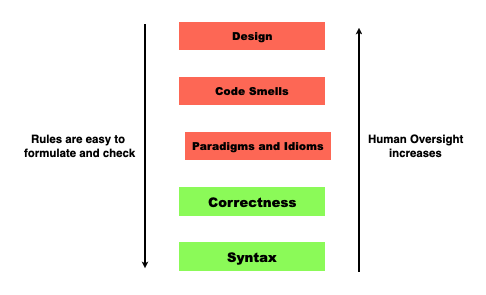
\includegraphics[width=\linewidth]{Figures/taxonomy.png}
    \caption{Hierarchy of software abstractions.}
    \label{fig:taxonomy}
\end{figure}

Based on our tests with Copilot shown in chapter~\ref{chapter:methodology}, Copilot was able to generate syntactically correct code that solves the given programming task in the coding scenario~(shown in ~\repl{}).
This functionality covers the syntax and the correctness level in our software abstraction hierarchy.
As a result, Copilot stands at the correctness level of our taxonomy. 

The challenges further up the hierarchy are nonetheless more important for software quality attributes (QA)~\cite{Ernst2017} and for a well-engineered software system.
For example, an automated solution suggested by \cct{} to the top level of the taxonomy would be able to follow heuristics to engineer a well-designed software system, which would be easy to modify and scale to sudden changes in use.